\section{Meditation of Thais}

\begin{wrapfigure}{rt}{.3\textwidth}
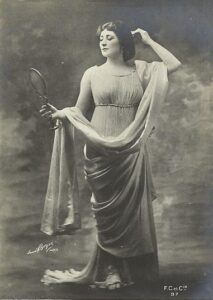
\includegraphics[width=.25\textwidth]{Thais-213x300.jpg}
\end{wrapfigure}

\paragraph{Me and God}

The 2009 movie \emph{The Answer Man\footnote{\url{https://www.imdb.com/title/tt1187041/}}} starts with an interesting premise but then deteriorates into a saccharine boy meets, loses, regains girl story. Arlen Faber wrote a best selling spiritual book titled \emph{Me and God}, in which he poses questions to God and records the responses. This led to spinoffs like the ``Me and God Diet'', ``Me and God for Teens'', etc. A cultlike following arose from the books. Arlen, however, is reclusive and makes no public appearances. Actually, his persona is arrogant, flippant, cynical, and unfriendly.

That is supposed to be off-putting, but it is actually endearing. He refuses to play the role of a spiritual guru gazing off into the Infinite. When it counts, however, he is kind; he took care of his Alzheimer diseased father in his final days. Nor does he live extravagantly although he could, and he lives a celibate life.

In a reversal of traditional wisdom, God was useless in Arlen's life. Only his new girlfriend could save him from himself.

\paragraph{The Master's Voice}


\begin{quotex}
The sheep hear his voice, and he calls his own sheep by name and leads them out. When he has brought out all his own, he goes before them, and the sheep follow him, for they know his voice.
\flright{\textsc{John 20:3-4}}
\end{quotex}


The mind of the masses is by nature inchoate. A leader is the one who is able to articulate their thoughts; they then recognize his voice. But the Good Shepherd calls out his own from among the masses. That is the voice that they recognize. Many are called but few are chosen. The rest have gone astray.

The film shows how an articulate voice can inspire the masses. In a scene at a bookstore, he implies that the authors of such books are more interested in the sales figures. In ``real life'', Arlen is mocking figures like Rick Warren, Eckhart Tolle, Neal Walsch, and others like them, who not only sell books but run expensive seminars.

\paragraph{Vedantic Christianity}


Edward Feser picks a fight with the latest book of his nemesis David Bentley Hart\footnote{\url{https://www.thepublicdiscourse.com/2022/03/80430/}}. Hart. DBH defends a position he calls Vedantic Christianity which he vehemently opposes to Thomism. Feser defends Saint Thomas and criticizes DBH for talking about God.

They are both weak on modal logic. Feser seems to believe that free will is the gnomic will, or the ability to make a choice.

\textbf{Objection 1}: Either the choice is arbitrary, in which case it is unfitting to God. Or the choice depends on some other factor, in which case God is not free.

DBH claims that the world follows necessarily from God's nature.

\textbf{Objection 2}: Free will means a will that arises from one's nature and is not dependent on something else. Hence, God's will does not depend on the world. The world therefore is not necessary since it is contingent on God's will.

\textbf{We answer that}: The fellows missed the mess call and are eating crumbs. Evola called Guido De Giorgio a ``Vedantic Christian''\footnote{\url{https://www.gornahoor.net/?p=1267}}.

Moreover, in \emph{Man and his Becoming}, Rene Guenon described the metaphysics of the Vedanta and asserted that in essential ways, Aristotle and the Scholastics were in harmony with that metaphysics.

\paragraph{Professional Thinkers}


The rise of the Internet has given rise to a new type of professional Christians and public intellectuals. 100K views on youtube can bring the author as much as \$1800; that does not count income from Patreon or superchats. The masses cannot juggle too many ideas at once, so these professionals have to repeat themselves. Once they have an image, it is costly to change it.

\paragraph{Jordan Peterson's IQ}


The fellow is obsessed with IQ and in a recent video he announces his IQ. The GRE used to be a good proxy for IQ. Me. Peterson says he scored in the 75\textsuperscript{th} percentile on the quantitative part of the test and that somehow equates to a 150 IQ. Now a person at that level of intelligence will be incomprehensible to the masses, even most college graduates. Or perhaps he is so intelligent that he understands that the masses will understand metaphors about lobsters and cleaning up your room.

He seems to almost megalomaniacal, claiming expertise on virtually any subject. Pseudo-intellectuals are recognized by their obsession with quantum mechanics, and that seems to be his most recent obsession.

\paragraph{Why ask why}


I often get very nice feedback from readers who understand what is going on here. Casual readers think we are encouraging a debating society. The Why of things are not amenable to debate. For example, an encyclopedic article on glass would describe its chemical composition, its history, its production. But the real question is ``why is there glass?'' It's really convenient that such a substance exists in the world.

\paragraph{Superimposition of Thought}


Intuition is a direct experience of the world, unmediated by thought. Its most basic form it is our sensual experience of the world, which is the fundamental form of knowing. We have a direct representation of the world in consciousness, which is prior to thinking. This then is covered up with a series of running thoughts, or ``narrative'' as it is called. This interpretation of reality displaces direct experience, as the commentary displaces the direct experience.

The \emph{ratio} is the first moment of the mind, but there is a higher form of knowing than that. Analogous to sense experience, there is direct, unmediated experience of higher realities. That is called ``intuition''. But even more noticeably, intuitions are mediated by running thoughts from theories, debates, etc. No matter how subtle the theories are, they can never achieve intuitive knowledge. Esoteric training requires mastery of the thinking function.

\paragraph{Thinking and Science}


If thinking and science are all that is required, why have all problems not been resolved by now? Of the approximately 50 billion humans who have ever existed, only an insignificant number have contributed anything of value to the human race beyond their own progeny.

\paragraph{Knowledge of the Gods}


From the above, it is obvious that the human race could never have survived in the wild. What are called ``primitive people'' are not an early phase of human existence. Rather, they are the residues of higher civilizations.

Civilization, and the technological means to achieve it, came from a higher source. There are competing theories about how that happened. The Hollywood version is that aliens from intergalactic civilizations brought that knowledge to earthlings. Occultists claim that ascended masters taught such things to the elites of the human race. The \emph{Book of Enoch} claims that angels brought technology:


\begin{quotex}
Azazel taught men to make swords, and knives, and shields, and breastplates, and made known to them the metals of the earth and the art of working them, and bracelets, and ornaments, and the use of antimony, and the beautifying of the eyelids, and all kinds of costly stones, and all colouring tinctures.
\end{quotex}


But the human race became corrupt, and knowledge became more ambiguous, with the possibility of evil. Enoch continues:

\begin{quotex}
There arose much godlessness, and they committed fornication, and they were led astray, and became corrupt in all their ways. Semjaza taught enchantments, and root-cuttings, Armaros the resolving of enchantments, Baraqijal, taught astrology, Kokabel the constellations, Ezeqeel the knowledge of the clouds, Araqiel the signs of the earth, Shamsiel the signs of the sun, and Sariel the course of the moon.
\end{quotex}


So the gods were reluctant to reveal too much, too soon. \textbf{Prometheus} had to steal knowledge from the gods, for which he was punished. We today benefit from our technology, yet are punished for knowing it.

\paragraph{Meditation de Thaïs}


Athanaël, a Cenobite monk, confronts Thaïs, a beautiful and hedonistic courtesan and devotée of Venus, and attempts to persuade her to leave her life of luxury and pleasure and find salvation through God. Following the Meditation, Thaïs tells Athanaël that she will follow him to the desert.

\url{https://www.youtube.com/watch?v=AfOAxQyuEUs} 

\flrightit{Posted on 2022-04-19 by Cologero}
